\documentclass[a4paper, 25pt]{article}
\usepackage[utf8]{inputenc}
\usepackage[english,russian]{babel}
\usepackage{amsmath,amssymb,amsfonts,textcomp,latexsym,amsopn}
\usepackage{cite,enumerate,float,indentfirst}
\usepackage{graphicx,xcolor}
\begin{document}

\begin{flushright}
Кобзарев Алексей, Тескер Константин, Белозёров Михаил, Рыбаков Владислав.
\\
410 группа
\end{flushright}

\begin{center}
\bfseries ОТЧЕТ ПО ПРАКТИКУМУ НА ЭВМ
\end{center}

\section{Постановка задачи}

Была поставлена задача написания программы проводящей расчёт течения в каверне разностной схемой. 
Система уравнений, описывающая нестационарное движение баротропного газа в область $\Omega$ размерности два, выглядит следующим образом

\begin{equation}
% \frac{\partial p}{\partial t} + div(\rhou) = 0,\\
 \rho[\frac{\partial u}{\partial t} + (u, \bigtriangledown)u]  + \bigtriangledown p = Lu + \rho f, ~~
 p = p (\rho).
\end{equation}
где $L$ есть линейный симметричный положительно определенный оператор.

В данном случае рассматривалась схема описывающая поведение плотности и скорости газа в каверне.

\section{Гладкое решение}

Для проверки правильности формул и работы программы были проведены тесты на гладком решении. В качестве гладкого решения для плотности и скорости были выбраны следующие функции:

$$u1 = sin (2x) * sin (2y) * e^t$$
$$u2 = sin (2x) * sin (2y) * e^{-t}$$
$$\rho = (cos (2x) + 1.5) * (sin (2y) + 1.5) * e^t$$


Для проверки решения далее приведены значения норм разности решения и действительного значения для различных сеток, а также таблица времени работы программы.

\begin{center}
 $C$-норма ошибки для $g: \quad p_{\rho}=10.000, \mu = 0.010 $
\begin{tabular}{|p{0.6in}|p{0.7in}|p{0.7in}|p{0.7in}|p{0.7in}|} \hline
$\tau\setminus h$ & $0.05$ & 0.025& 0.0125 & 0.00625 \\ \hline
$0.00200$ & $5.448e-02$ &$1.294e-01$ &$1.553e-01$ &$1.596e-01$  \\ \hline
$0.00100$ & $5.411e-02$ &$1.298e-01$ &$1.559e-01$ &$1.602e-01$  \\ \hline
$0.00050$ & $5.392e-02$ &$1.301e-01$ &$1.562e-01$ &$1.606e-01$  \\ \hline
$0.00025$ & $5.383e-02$ &$1.302e-01$ &$1.563e-01$ &$1.607e-01$  \\ \hline
\end{tabular}\\[20pt]
\end{center}

\begin{center}
 $L_2$-норма ошибки для $g: \quad p_{\rho}=10.000, \mu = 0.010 $
\begin{tabular}{|p{0.6in}|p{0.7in}|p{0.7in}|p{0.7in}|p{0.7in}|} \hline
$\tau\setminus h$ & $0.05$ & 0.025& 0.0125 & 0.00625 \\ \hline
$0.00010$ & $2.870e-03$ &$3.513e-03$ &$3.662e-03$ &$3.630e-03$  \\ \hline
$0.00005$ & $2.869e-03$ &$3.513e-03$ &$3.662e-03$ &$3.630e-03$  \\ \hline
$0.00003$ & $2.868e-03$ &$3.513e-03$ &$3.662e-03$ &$3.630e-03$  \\ \hline
$0.00001$ & $2.868e-03$ &$3.513e-03$ &$3.662e-03$ &$3.630e-03$  \\ \hline
\end{tabular}\\[20pt]
\end{center}

\begin{center}
$C$-норма ошибки для $v1: \quad p_{\rho}=10.000, \mu = 0.010 $
\begin{tabular}{|p{0.6in}|p{0.7in}|p{0.7in}|p{0.7in}|p{0.7in}|} \hline
$\tau\setminus h$ & $0.05$ & 0.025& 0.0125 & 0.00625 \\ \hline
$0.00010$ & $3.113e-02$ &$2.139e-02$ &$2.264e-02$ &$4.636e-02$  \\ \hline
$0.00005$ & $3.113e-02$ &$2.139e-02$ &$2.264e-02$ &$4.636e-02$  \\ \hline
$0.00003$ & $3.113e-02$ &$2.139e-02$ &$2.264e-02$ &$4.636e-02$  \\ \hline
$0.00001$ & $3.113e-02$ &$2.139e-02$ &$2.264e-02$ &$4.636e-02$  \\ \hline
\end{tabular}\\[20pt]
\end{center}

\begin{center}
 $L_2$-норма ошибки для $v1: \quad p_{\rho}=10.000, \mu = 0.010 $
\begin{tabular}{|p{0.6in}|p{0.7in}|p{0.7in}|p{0.7in}|p{0.7in}|} \hline
$\tau\setminus h$ & $0.05$ & 0.025& 0.0125 & 0.00625 \\ \hline
$0.00010$ & $1.678e-02$ &$1.060e-02$ &$7.112e-03$ &$4.020e-03$  \\ \hline
$0.00005$ & $1.656e-02$ &$1.060e-02$ &$7.112e-03$ &$4.020e-03$  \\ \hline
$0.00003$ & $1.656e-02$ &$1.060e-02$ &$7.113e-03$ &$4.020e-03$  \\ \hline
$0.00001$ & $1.656e-02$ &$1.060e-02$ &$7.113e-03$ &$4.021e-03$  \\ \hline
\end{tabular}\\[20pt]
\end{center}

\begin{center}
 $C$-норма ошибки для $;v2: \quad p_{\rho}=10.000, \mu = 0.010 $
\begin{tabular}{|p{0.6in}|p{0.7in}|p{0.7in}|p{0.7in}|p{0.7in}|} \hline
$\tau\setminus h$ & $0.05$ & 0.025& 0.0125 & 0.00625 \\ \hline
$0.00010$ & $1.928e-02$ &$2.098e-02$ &$3.527e-02$ &$5.971e-02$  \\ \hline
$0.00005$ & $2.286e-02$ &$2.098e-02$ &$3.527e-02$ &$5.971e-02$  \\ \hline
$0.00003$ & $2.286e-02$ &$2.098e-02$ &$3.528e-02$ &$5.971e-02$  \\ \hline
$0.00001$ & $2.286e-02$ &$2.098e-02$ &$3.528e-02$ &$5.971e-02$  \\ \hline
\end{tabular}\\[20pt]
\end{center}

\begin{center}
$L_2$-норма ошибки для $v2: \quad p_{\rho}=10.000, \mu = 0.010  $
\begin{tabular}{|p{0.6in}|p{0.7in}|p{0.7in}|p{0.7in}|p{0.7in}|} \hline
$\tau\setminus h$ & $0.05$ & 0.025& 0.0125 & 0.00625 \\ \hline
$0.00010$ & $4.887e-03$ &$2.924e-03$ &$1.816e-03$ &$2.299e-03$  \\ \hline
$0.00005$ & $5.464e-03$ &$2.924e-03$ &$1.816e-03$ &$2.300e-03$  \\ \hline
$0.00003$ & $5.464e-03$ &$2.924e-03$ &$1.816e-03$ &$2.300e-03$  \\ \hline
$0.00001$ & $5.464e-03$ &$2.924e-03$ &$1.816e-03$ &$2.300e-03$  \\ \hline
\end{tabular}\\[20pt]
\end{center}

\begin{center}
Время, $p_{\rho}=10.000, \mu = 0.010  $
\begin{tabular}{|p{0.6in}|p{0.7in}|p{0.7in}|p{0.7in}|p{0.7in}|} \hline
$\tau\setminus h$ & $0.05$ & 0.025& 0.0125 & 0.00625 \\ \hline
$0.00010$ & $8.603e-03$ &$2.935e-02$ &$1.295e-01$ &$7.603e-01$  \\ \hline
$0.00005$ & $1.550e-02$ &$5.310e-02$ &$2.467e-01$ &$1.341e+00$  \\ \hline
$0.00003$ & $3.005e-02$ &$9.889e-02$ &$4.552e-01$ &$2.554e+00$  \\ \hline
$0.00001$ & $5.630e-02$ &$1.962e-01$ &$8.307e-01$ &$4.615e+00$  \\ \hline
\end{tabular}\\[20pt]
\end{center}


Результаты свидетельствуют о том, что программа реализована верно и имеет место сходимость решения к действительному значению плотности и скорости.
\newpage

\section {Численные эксперименты}

Были проведены численные эксперименты, моделирующие реальных условий.
Блыли реализованы четыре версии программы описываще различные по форме каверны.
Начальные условия были установлены следующие:
Белозёров Михаил
\begin {itemize}
\item Область $\Omega = \Omega_{02} \cup \Omega_{12} \cup \Omega_{22} \cup \Omega{11} \cup \Omega{21} \cup \Omega{10} \cup \Omega_{20}$
  \item $u_1|_{\Gamma_{02}^{x-}} = \omega$
  \item $\frac{{\partial}u_2}{{\partial}y}|_{\Gamma_{10}^{y-}\cup\Gamma_{20}^{y-}} = 0$
\end   {itemize}

Для выяснения корректности проведенных экспериментов была написана дополнительная программа, визуализирующая результаты проделанных экспериментов. Было замечено, что при увеличении временного парметра решение стабилизируется и результаты для каждой из задач выглядят следующим образом: \\
\begin{figure}[h!]
\center{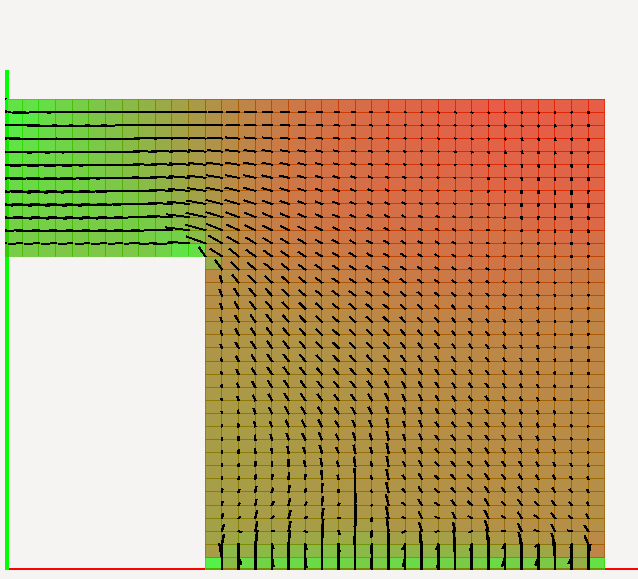
\includegraphics[width=1\linewidth]{screen_belozerov.jpg}}
\end{figure}
\\
Плотность газа характеризуется цветом ячейки. От зелёного к красному по возрастанию значения плотности. Черные палочки -- вектора скорости.

\section{Сходимость и собственные функции}
Были проведены эксперименыты по скорости сходимости для изначального решения. Результаты приведены ниже.

Для матрицы были вычислено время установления стационарного решения и время восстановления его после возмущения.
К сожалению на данный момент найти собственный вектор для данной матрицы не удалось поэтому возмущение проводилось случайным образом в пределах от $-0.1$ до $ 0.1$ \\
Для $\tau = 3.125000e-02$ и $ h = 1.047198e+00 $ \\
Время выхода на стационарное решение составило $38$cекунд.\\
Время выхода на стационарное решение после возмущения составило $1.406250$ секунд.\\
Для тех же $\tau, h$ и значения случайной функции от $-0.3$ до $ 0.3$ \\
Время выхода на стационарное решение составило $38$cекунд.\\
Время выхода на стационарное решение после возмущения составило $11.562500$ секунд.\\
\section{Описание реализации}
Программа реализована на языке С, опираясь на исходный код выданной программы и используя пакет laspack.
Для реализации были созданы масивы инндексирующие связь плотности и скорости. Массивы назваются left bottom v - индекс скорости стоящей на пол узла ниже и пол узла левее плотности.
left h index -  индекс плотности на полл узла правее и пол узла выше узла скорости
left top h index -  индекс плотности на полл узла левее и пол узла выше узла скорости

nак же для облегчения работы с индексами были ввеедены два массива hv map и vh map jтвечающие за соответствие узлов скорости и плотности.

Для реализации заполнения сетки и начальных данныхбыли написаны функции set arrays for H, reset H index, setka for v.\\
Схема решения притерпела небольшие изменения. Вместо одного вычисления матрицы размерности $DIM_H + 2 * DIM_V$ теперь используется две матрицы размерности $DIM_H$ для плотности  и размерности $2 * DIM_V$ для скорости. На каждом шаге по времени происходит сначала вычисление плотности по данным с предыдущего шага. Затем просиходит вычисление скорости по плотности с новго шага и значений сокрости с предыдущего шага. 

Для вычисления индексов для узла были добавлены функции fill for H и fill for v.
Для заполенения матриц использвуются функции cases H и case 0 V, case 1 8 V. Так как скорости на границах полагаются известными то разбирать случаи граничных узлов не имеет смысла, для них написан общий случай выставления диагонального элемента значение 1 и правой части с действительным значением скорости в этом узле.

\section{Заключение}
В результате проведенных экспериментов было установлено, что схема даёт правдивые результаты и может быть использована для расчётов реальных моделей течения газов. 
\end{document}
